\documentclass{article}  

\usepackage{times}
\usepackage{graphicx}
\usepackage{lipsum}  
\usepackage{xcolor}
\usepackage{fullpage}
\usepackage{xurl}
\usepackage{tabularx}
\usepackage{amsmath}
\usepackage{svg}
\usepackage{float}
\usepackage{parskip} % Removes paragraph indentation
\usepackage{listings}

\usepackage{xcolor}

\lstdefinelanguage{Cypher}{
  morekeywords={
    MATCH, RETURN, ORDER, BY, LIMIT, WHERE, CREATE, DELETE, SET, DETACH,
    WITH, MERGE, OPTIONAL, AS, AND, OR, NOT, IN, ON, FOREACH, CASE, WHEN, THEN, ELSE, END, DISTINCT
  },
  sensitive=true,
  morecomment=[l]{//},
  morestring=[b]',
}

\lstdefinestyle{cypherStyle}{
  language=Cypher,
  basicstyle=\ttfamily\small,
  keywordstyle=\color{blue}\bfseries,
  commentstyle=\color{gray}\itshape,
  stringstyle=\color{teal},
  numbers=left,
  numberstyle=\tiny\color{gray},
  stepnumber=1,
  numbersep=10pt,
  backgroundcolor=\color{gray!10},
  frame=single,
  tabsize=2,
  breaklines=true,
  breakatwhitespace=false,
  showstringspaces=false,
  captionpos=b
}

\lstdefinestyle{pythonStyle}{
  language=Python,
  basicstyle=\ttfamily\small,
  keywordstyle=\color{blue}\bfseries,
  commentstyle=\color{gray}\itshape,
  stringstyle=\color{teal},
  numbers=left,
  numberstyle=\tiny\color{gray},
  stepnumber=1,
  numbersep=10pt,
  backgroundcolor=\color{gray!10},
  frame=single,
  tabsize=4,
  breaklines=true,
  breakatwhitespace=false,
  showstringspaces=false,
  captionpos=b
}

\newcommand{\question}[1]{#1}

\title{Electric vehicle charging stations in the province of Zuid-Holland}
\author{Datasheet Authors: Dennis Hermann, Ivan Lee, Yih Fei Lim, Nikola Mitsev}

\begin{document}
\date{\today}
\maketitle

This datasheet was prepared following the ``Datasheets for Datasets'' template of Gebru et al.\ \cite{gebru}, extended where needed following the frameworks of Pushkarna et al.\ \cite{pushkarna} and Paullada et al.\ \cite{Paullada}.

%%%%%%%%%%%%%%%%%%%%%%%%%%%%%%%%%%%%%%%%%%%%%%%%%%%%%%%%%%%%%%%%%%%%%%%%%%%%%%%%
% \section{Question for the meeting}
% Does data exchange in this context refer to the process of translating from the data source format to the file format used for the knowledge graph? If so, what about manually transcribed data - what would data exchange entail here?
\section{Motivation For Data/Knowledge Creation}

\question{\subsubsection*{Why was the dataset/knowledge graph created? (e.g., was there a specific task in mind? was there a specific gap that needed to
		be filled?)}}

%\lipsum[1]
%The knowledge graph was created to find suitable and profitable locations for building new EV charging stations in the province of Zuid-Holland, based on the price of the land that would be required to build the station, the price of the electricity for the city/province, the number of rival companies charging stations and average salary which is used to determine regions where EV ownership might be in higher proportions than the average. (original text used for the prompt on copilot I just said can you turn these bullet points into a single text)
The knowledge graph was developed to identify optimal and profitable locations for establishing new electric vehicle (EV) charging stations in the province of Zuid-Holland. This analysis considers several key factors, including the cost of the land required to build the charging station, the price of electricity in the city or province, the number of existing charging stations operated by rival companies, and the average salary in different regions. By evaluating land prices, the knowledge graph helps pinpoint areas where the investment would be most cost-effective. Additionally, lower electricity costs can enhance the profitability of the charging stations. Analyzing the number of rival companies' charging stations helps avoid oversaturation and ensures a competitive edge. Furthermore, the average salary is used to estimate areas with potentially higher EV ownership rates, as higher income levels often correlate with a greater likelihood of EV adoption. By integrating these factors, the knowledge graph provides a comprehensive overview, enabling informed decisions on where to build new EV charging stations to maximize profitability and meet the growing demand for EV infrastructure.

\question{\subsubsection*{What (other) tasks could the dataset be used for?}}

%\lipsum[1]
City planners and private investors could use the datasets to identify suitable land for housing developments. By analyzing land prices and electricity costs, planners can pinpoint cities and areas where housing projects would be most cost-effective and attractive to potential residents. Lower land prices can reduce initial investment costs, while affordable electricity rates can make living in these areas more appealing. The knowledge graph could be used for smart grid optimization and energy infrastructure planning. Energy providers and policymakers can identify strategic zones for deploying grid-scale battery storage or renewable energy microgrids. However, the visualization tool would have to be updated accordingly to accommodate these tasks.

% \question{\subsubsection*{Any other comments?}}

% \lipsum[1]

\section{Dataset and Knowledge Graph Composition}

\question{\subsubsection*{What do the instances that comprise the dataset represent?(e.g., documents, images, people, countries) Are there multiple types
		of instances? (e.g., movies, users, ratings; people, interactions between them; nodes, edges)}}
In our knowledge graph, we have 4 types of nodes, each containing their own properties. They describe existing EV Charging Stations, as well as potential Candidate Locations which the client may look at. The EV Charging Stations and Candidate Locations are then located within a PC4Area which is then located within a Municipality.
\begin{table}[H]
	\begin{tabularx}{\textwidth}{l|l|X}
		\textbf{Node}     & \textbf{Key}             & \textbf{Value}                                                          \\
		\hline
		Municipality      & name                     & Municipality Name                                                       \\
		\cline{2-3}
		                  & addresses                & Total number of Addresses                                               \\
		\cline{2-3}
		                  & area                     & Total Area of the municipality in Hectares (0.01 km\textsuperscript{2}) \\
		\cline{2-3}
		                  & business\_establishments & Total number of Businesses                                              \\
		\cline{2-3}
		                  & dwellings                & Total number of Dwellings                                               \\
		\cline{2-3}
		                  & home\_value              & Average Home Value in the Municipality                                  \\
		\cline{2-3}
		                  & households               & Total number of Households                                              \\
		\cline{2-3}
		                  & passenger\_cars          & Total number of passenger cars                                          \\
		\cline{2-3}
		                  & persons\_per\_household  & Average number of persons per household                                 \\
		\cline{2-3}
		                  & population\_density      & Population Density                                                      \\
		\cline{2-3}
		                  & vehicles                 & Total number of vehicles                                                \\
		\hline
		PC4Area           & name                     & PC4 Code                                                                \\
		\cline{2-3}
		                  & geometry                 & The polygon shape of the PC4 area                                       \\
		\cline{2-3}
		                  & density                  & EV charger density of the PC4 per Hectare (0.01 km\textsuperscript{2})  \\
		\hline
		EVChargingStation & location                 & Coordinates of the Charging Station in SRID4326                         \\
		\cline{2-3}
		                  & nearest\_location        & Coordinates of the closest other Charging Station in SRID 4326          \\
		\cline{2-3}
		                  & distance\_to\_nearest    & Distance to the closest other Charging Station in m                     \\
		\hline
		CandidateLocation & location                 & Coordinates of the Candidate Location in SRID4326                       \\
		\cline{2-3}
		                  & nearest\_location        & Coordinates of the closest existing Charging Station in SRID 4326       \\
		\cline{2-3}
		                  & distance\_to\_nearest    & Distance to the closest existing Charging Station in m                  \\
		\cline{2-3}
		                  & score                    & Score calculated based on formula                                       \\
		\hline
	\end{tabularx}
	\caption{Table of Nodes and their Properties}
	\label{table:nodesandproperties}
\end{table}

\begin{figure}[H]
	\centering
	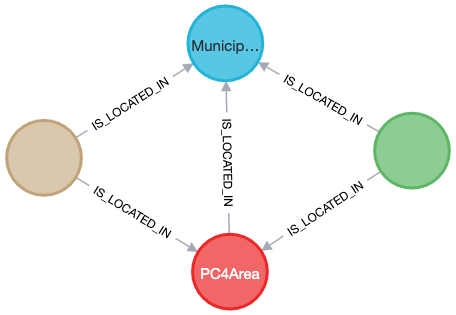
\includegraphics[width=0.5\linewidth]{graph.png}
	\caption{Meta Graph of our knowledge graph. Blue: Municipality, Red: PC4Area, Brown: EVChargingStation, Green: CandidateLocation}
	\label{fig:meta-graph}
\end{figure}

\question{\subsubsection*{How many instances are there in total (of each type, if appropriate)?}}
\begin{table}[H]
	\begin{tabularx}{\textwidth}{X|X}
		\textbf{Node}     & \textbf{Count} \\
		\hline
		Municipality      & 50             \\
		\hline
		PC4Area           & 542            \\
		\hline
		EVChargingStation & 9226           \\
		\hline
		CandidateLocation & 43083          \\
		\hline
	\end{tabularx}
	\caption{Number of Nodes in Graph}
\end{table}

\question{\subsubsection*{What data does each instance consist of ? “Raw” data (e.g., unprocessed text or images)? Features/attributes? Is there a label/target associated with
		instances? If the instances related to people, are subpopulations identified (e.g., by age, gender, etc.) and what is
		their distribution?}}
Each EVChargingStation represents an actual Charging Location as described by the OpenStreetMap and/or OpenChargeMap APIs.

Each CandidateLocation represents a Parking Lot as described in the OpenStreetMap API.

Each PC4Area represents a PC4 Postal Code in Zuid-Holland, with a corresponding Polygon, so that we can search if any of the other locations are also in the PC4 Area.

Each Municipality represents a Municipality in Zuid-Holland. As the largest administrative division we are looking at in our data, this includes all the additional properties that we gathered in Table \ref{table:nodesandproperties}.

\question{\subsubsection*{Is any information missing from individual instances? If so, please
		provide a description, explaining why this information is missing (e.g., because it was unavailable). This does not include intentionally removed information, but might include, e.g., redacted text.}}
No, none of the data we required was missing.

\question{\subsubsection*{Are relationships between individual instances made explicit (e.g.,
		users’ movie ratings, social network links)? If so, please describe
		how these relationships are made explicit.}}
Yes, we made edges to denote which nodes are located within which other nodes, such as PC4Area and Municipality. Although the Municipality that a CandidateLocation or EVChargingStation is in could be queried based on the PC4Area it is in, we additionally added an explicit edge to denote that the relevant location is located within the Municipality. This can be observed in Figure \ref{fig:meta-graph}

\question{\subsubsection*{Does the dataset contain all possible instances or is it a sample (not
		necessarily random) of instances from a larger set (bootstrapping)? If the dataset is
		a sample, then what is the larger set? Is the sample representative of the
		larger set (e.g., geographic coverage)? If so, please describe how this
		representativeness was validated/verified. If it is not representative of the
		larger set, please describe why not (e.g., to cover a more diverse range of
		instances, because instances were withheld or unavailable).}}
Our dataset is complete, as we have found that the size of the data was manageable within our means. This includes all existing EV Charging Stations, Parking Lots and data about Municipalities in Zuid-Holland.

\question{\subsubsection*{Are there recommended data splits (e.g., training, development/validation, testing)? If so, please provide a description of these splits, explaining the rationale behind them.}}
No we recommend using the whole dataset together when calculating the scores to ensure the best robustness.

\question{\subsubsection*{Are there any errors, sources of noise, or redundancies in the dataset? If so, please provide a description.}}
As the EV Charging Stations and Candidate Locations come from crowdsourced datasets like OpenStreetMap and OpenChargeMap, these may have some noise, because of human input error. Since we are using redundant datasets as well, from both APIs, some EV Charging Stations may be represented twice. However, this is rectified by the process in \ref{subsubsection:contradictions}

\question{\subsubsection*{Is the dataset self-contained, or does it link to or otherwise rely on
		external resources (e.g., websites, tweets, other datasets)? If it links
		to or relies on external resources, a) are there guarantees that they will
		exist, and remain constant, over time; b) are there official archival versions
		of the complete dataset (i.e., including the external resources as they existed at the time the dataset was created); c) are there any restrictions
		(e.g., licenses, fees) associated with any of the external resources that
		might apply to a future user? Please provide descriptions of all external
		resources and any restrictions associated with them, as well as links or
		other access points, as appropriate.}}
Once published, the dataset is self-contained and can be used as is. However, it can be updated when the client decides to build a new charging station, or when the client wants to refresh the data from the sources.

To update the data, code to utilise the OpenStreetMap and OpenChargeMap APIs are provided to the client.

As OpenChargeMap uses the CreativeCommons License, it is free to use and adapt as long as there is attribution. Similarly OpenStreetMap uses the Open Data Commons Open Database License which is also free to use as long as there is attribution.

The PC4 Geojson is maintained by the Government of the Netherlands and we found the source from OpenDataSoft, which is a repository of Governmental Data across Europe.

Finally AlleCijfers is a data aggregator and has provided a list of all its sources used, which allows our client to piece it together in the future even if AlleCijfers stops operating or updating the dataset.

% \question{Any other comments?}

\section{Collection Process}
% Suggestion:
For each of the datasets you have collected and integrated to answer your client's knowledge request, please answer the following questions. You can give each dataset a name and refer to it by that name.

\question{\subsubsection*{(If you did not record the data yourself) Where did you download the data from? Please elaborate on why this is an appropriate source.    Has the dataset been used already? If so, where are the results so others can compare
		(e.g., links to published papers)? Who funded the creation dataset?}}
\begin{itemize}
	\item \textbf{PC4 GeoJSON} \\
	      \textit{Source:} Downloaded from publicly available open-data repositories that provide GeoJSON polygon data for PC4 areas in the Netherlands. \\
	      \textit{Appropriateness:} This dataset is suitable as PC4 postcodes are widely used in spatial analysis within the Netherlands. \\
	      \textit{Usage and Funding:} PC4 GeoJSON files are widely used in spatial research, urban planning, and public sector analysis.

	\item \textbf{OpenStreetMap API} \\
	      \textit{Source:} OpenStreetMap (OSM), accessible via their public API. \\
	      \textit{Appropriateness:} OSM is a global, crowdsourced geospatial database known for its high accuracy and community-driven updates. It provides both existing and candidate charger locations, making it suitable as our primary charger location source. \\
	      \textit{Usage and Funding:} OSM data has been used extensively in many academic and commercial projects. It is maintained by a community of volunteers via open collaboration.

	\item \textbf{OpenChargeMap API} \\
	      \textit{Source:} OpenChargeMap (OCM), accessible via their public API. \\
	      \textit{Appropriateness:} OCM specializes in electric vehicle charger data, making it highly appropriate as a secondary (redundant/backup) source for charger locations to cross-validate OSM data. \\
	      \textit{Usage and Funding:} OpenChargeMap data is used in various EV charging apps and research projects. The platform data is crowd-sourced by their users and those of apps that use OCM data.

	\item \textbf{AlleCijfers.nl} \\
	      \textit{Source:} AlleCijfers.nl, which aggregates Dutch municipal socio-economic and demographic data from official sources like CBS (Statistics Netherlands). \\
	      \textit{Appropriateness:} Provides reliable, up-to-date demographic and socio-economic data for each municipality, crucial for understanding population density, income levels, and vehicle density that lets us gain insights on the EV Charger demand in the area. \\
	      \textit{Usage and Funding:} AlleCijfers.nl data is widely used by policy makers, researchers, and local governments. The underlying data originates from official government-funded statistics agencies.

	\item \textbf{Google Maps Geocoding API} \\
	      \textit{Source:} Google Cloud Platform’s Geocoding API service. \\
	      \textit{Appropriateness:} Used for reverse geocoding PC4 postcodes to municipality names, enabling linkage of postcode-based spatial data to municipality-level socio-economic datasets. \\
	      \textit{Usage and Funding:} Google’s geocoding API is used in both commercial and academic spatial applications. It is provided by Google as part of its commercial cloud services.
\end{itemize}

\question{\subsubsection*{(If you did record the data yourself) What mechanisms or procedures were used to collect the data (e.g.,
		hardware apparatus or sensor, manual human curation, software program, software API)? How were these mechanisms or procedures validated?}}
We did not record any data ourselves.

\question{\subsubsection*{How was the data associated with each instance acquired? Was the
		data directly observable (e.g., raw text, movie ratings), reported by subjects (e.g., survey responses), or indirectly inferred/derived from other data
		(e.g., part-of-speech tags, model-based guesses for age or language)?
		If data was reported by subjects or indirectly inferred/derived from other
		data, was the data validated/verified? If so, please describe how.}}
\subsubsection*{Data Acquisition and Validation}

\begin{itemize}
	\item \textbf{PC4 GeoJSON:} Directly observed geographical boundaries from official Dutch government sources (e.g., CBS).

	\item \textbf{OpenStreetMap API:} Directly observed charger locations contributed by users and organizations; validated through community reviews.

	\item \textbf{OpenChargeMap API:} Subject-reported charger data from users and apps; validated through community moderation.

	\item \textbf{AlleCijfers.nl:} Directly observed socio-economic and demographic statistics from official government registers (CBS), ensuring high accuracy.

	\item \textbf{Google Maps Geocoding API:} Indirectly inferred municipality names via reverse geocoding algorithms maintained and updated by Google.
\end{itemize}

\question{\subsubsection*{If the dataset is a sample from a larger set, what was the sampling strategy (e.g., deterministic, probabilistic with specific sampling probabilities)?}}
We did not engage in sampling of data

\question{\subsubsection*{Who was involved in the data collection process (e.g., students,
		crowdworkers, contractors) and how were they compensated (e.g.,
		how much were crowdworkers paid)? What does this context mean for your project?}}
\subsubsection*{Who was involved in the data collection process and how were they compensated? What does this context mean for your project?}

The data collection involved multiple independent entities:

\begin{itemize}

	\item \textbf{PC4 GeoJSON:} Source was made available by OpenDataSoft, a French company specialising in data. Employees involved in this were likely compensated through their salaries.

	\item \textbf{AlleCijfers.nl:} Collected by government agencies using official administrative registers. Government employees were compensated through public sector salaries.

	\item \textbf{OpenStreetMap:} Data was contributed by volunteers and organizations on a voluntary basis without direct compensation, as part of a global crowdsourcing initiative.

	\item \textbf{OpenChargeMap:} Contributions were made by volunteers. Most contributors were likely uncompensated.

	\item \textbf{Google Maps Geocoding API:} Provided as a paid cloud service by Google.

\end{itemize}

For our project, this means the data come from a combination of highly reliable official sources but also community-driven platforms, which may include some variability in accuracy, particularly for charger locations.

\question{\subsubsection*{What was the motive behind capturing the data? What does this context mean for your project?}}

The original motives vary by source:

\begin{itemize}
	\item \textbf{PC4 GeoJSON}: Collected to further the company (i.e. OpenDataSoft) in its data sharing mission.

	\item \textbf{AlleCijfers.nl:} Collected for aggregating stats for national statistics, urban planning, and policy making.

	\item \textbf{OpenStreetMap:} Built as an open, free, and global map database for public use.

	\item \textbf{OpenChargeMap:} Created to provide open access to electric vehicle charging station map and data for EV drivers and developers.

	\item \textbf{Google Maps Geocoding API:} Built to support geocoding and location-based services for commercial and developer applications.

\end{itemize}

These motives align well since our goal is to analyze and model EV charger availability using accurate spatial and demographic data.

\question{\subsubsection*{Where was the data recorded? (geographic location, time, sociological context and possible others.) What does this context mean for your project?}}

All data was recorded within the Netherlands:

\begin{itemize}
	\item \textbf{PC4 GeoJSON and AlleCijfers.nl:} National coverage of the Netherlands.
	\item \textbf{OpenStreetMap and OpenChargeMap:} Charger locations within the Netherlands.
	\item \textbf{Google Maps Geocoding API:} Used for mapping Dutch postcode areas to municipalities.
\end{itemize}

\question{\subsubsection*{Over what timeframe was the data collected? Does this timeframe
		match the creation timeframe of the data associated with the instances (e.g., recent crawl of old news articles)? If not, please describe the timeframe in which the data associated with the instances was created.}}
The data was collected between March 2025 and May 2025 as part of this project. The collection timeframe largely overlaps with the creation timeframe of the data; each data source contain data which are maintained and up to date.

\question{\subsubsection*{Who was the data created for? What does this context mean for your project?}}

\begin{itemize}
	\item \textbf{PC4 GeoJSON and AlleCijfers.nl:} Created for government, researchers, policy makers, and the general public.
	\item \textbf{OpenStreetMap:} Created for open public use by anyone needing spatial data.
	\item \textbf{OpenChargeMap:} Created for EV drivers, charging networks, developers, and researchers in the EV field.
	\item \textbf{Google Maps Geocoding API:} Created for commercial and developer use cases requiring geocoding services.
\end{itemize}

This diverse intended audience supports the multi-purpose nature of our project specific intended use cases.

\question{\subsubsection*{Is there a research question associated with the original dataset, and if yes, what is it? If no, what could be the reason for sharing the data? What does this context mean for your project?}}
\lipsum[1]
Most original datasets were not collected for a specific research question but serve general mapping, statistical reporting, or infrastructure documentation purposes. For example:

\begin{itemize}
	\item \textbf{PC4 GeoJSON and AlleCijfers.nl:} Collected for national statistics and administrative purposes.
	\item \textbf{OpenStreetMap and OpenChargeMap:} Built as open data platforms for broad community and developer usage.
	\item \textbf{Google Maps Geocoding API:} Provided as a general-purpose location service as part of Google Cloud services.
\end{itemize}

Our project leverages these datasets to address our own research questions around potential EV charger

\section{Data Transformation and Presentation}

\question{\subsubsection*{Was the “raw” data saved in addition to the preprocessed/cleaned/labeled data (e.g., to support unanticipated future uses)? If so, please provide a link or other access point to the “raw” data.}}

From the PC4\footnote{PC4 code is the Postal Code in the Netherlands with the 2 suffix letters removed, denoting a larger geographical area.} geojson dataset, we can obtain all the vertices which denote the polygon of the PC4 area and use it for the OSM query. Since postal codes are typically static and do not change for long durations, we have downloaded the dataset for use in its raw form. However we do maintain a link to the source in the event that postal districts are reworked.

For the charging station data and possible new charger locations, we are currently using the overpass API provided by OpenStreetMap (OSM), to gather the data per PC4 area. Since OpenStreetMap gets regularly updated from time to time, we will regularly pull the latest data for the area from the API as and when we query or update the knowledge graph.

As a backup and redundant data source, we will also incorporate the OpenChargeMap (OCM) API to retrieve another list of existing charging station locations. Similarly we will store the information locally, but with regular updates from the API when we update or query the knowledge graph.

Building upon the above data sources, we will also incorporate information from AlleCijfers, a platform that consolidates data from multiple official sources. Specifically, we can obtain detailed demographic and socio-economic data for each of the 50 municipalities within Zuid-Holland. In contrast to other sources, the dataset does not offer downloadable options. Instead, we extracted the figures manually in a structured format (i.e. CSV file) for reproducability.

\begin{table}[htbp]
	\begin{tabularx}{\textwidth}{l|X}
		\textbf{Data}                   & \textbf{Source URL}                                                                          \\
		\hline
		PC4 Geojson                     & \url{https://public.opendatasoft.com/explore/dataset/georef-netherlands-postcode-pc4/table/} \\
		OpenStreetMap API documentation & \url{https://wiki.openstreetmap.org/wiki/Overpass_API}                                       \\
		OpenChargeMap API documentation & \url{https://openchargemap.org/site/develop/api}                                             \\
		AlleCijfers                     & \url{https://allecijfers.nl/provincie/zuid-holland/#tabel_gebieden}
	\end{tabularx}
	\caption{Table of raw data sources/API documentations}

\end{table}

\question{\subsubsection*{Which degree of interaction with the data was needed to prepare the data? (Discovery, Capture, Curation, Design, Creation)}}
To work with the charging location and possible location data, we had to augment it with additional information. For the information gathered from the OSM queries, since we are querying for it on a PC4 level, we add the property that this specific chargers are in the corresponding PC4 area. However, since OCM works based on a rectangular bounding box, we have to write an additional function to map from latitude and longitude coordinates into the correct PC4 area.

Once PC4s have been tagged to each charging location in Zuid-Holland, we then have to calculate a charger density per PC4 area, by taking the number of chargers in each PC4 and dividing by its total area.
$$
	\text{Charger Density} = \frac{\text{No. of Chargers in PC4}}{\text{Area of PC4}}
$$

We also want to take into account the number of existing charging stations within a set radius around the potential locations. To do so, we check the distance between the potential locations and the existing chargers coordinates and enumerate for each location found.

Since AlleCijfers does not provide a downloadable dataset, we manually extracted key municipality-level statistics (e.g., population, area, income) directly from the website. This manual curation involved transcribing data into structured files for integration with our spatial and charger datasets, representing a higher degree of capture and creation interaction compared to automated sources.

Key properties such as home value, population density and vehicle density of each municipality are manually extracted from the dataset. Similar to other datasets, metrics regarding density are calculated by dividing the raw count by the land area of the municipality.

\[
	\text{Population Density} = \frac{\text{Population}}{\text{Land Area}} \quad ; \quad
	\text{Vehicle Density} = \frac{\text{Number of Vehicles}}{\text{Land Area}}
\]

\question{\subsubsection*{Did you find contradictions in your data? If yes, how did you deal with them?}}
\label{subsubsection:contradictions}
Since we are using 2 publicly collated data sources to gather our charging station information, means that there are bound to be some data points which are present in one but not the other. On the surface value this may seem like a contradiction, but is most likely due to the ad hoc nature of data collection for OSM and OCM. Since it is unfeasible for us to map out all the charging stations in Zuid-Holland ourselves to verify, we will be assuming that all charging stations in both data sources exist.

However, to prevent double counting certain stations and be as robust as possible, we will use the latitude and longitude data to match up the charging stations within 2m of each other as the same location. And accept them even if it only appears in one of the sources. This ensures our charging station data is as complete as possible without accidentally padding extra charging stations.

\question{\subsubsection*{Did you find conflicts in your data? If yes, how did you deal with them?}}
Due to the limited relevant data sources available, we were not able to find any contradictions as each data source was mutually exclusive from another.

\question{\subsubsection*{How did you organize your data? Describe the categorization and/or classification of your data set. Feel free to include diagrams or other imagery.}}
Since we are dealing in the geospatial domain, one of our main categories of data is geospatial in nature. This includes our charging station data, demographic data and socio-economic data.

However, to be more fine grained, our data can be further sub-divided into those with specific coordinates, or those aggregated on larger PC4 areas or municipality levels.

We wanted to make sure that all our data could be linked together in a knowledge graph like structure, with edges mapping to properties in other datasets, which is why we intend to map all coordinates to PC4 regions, which are then mapped to the various municipalities in Zuid-Holland. More of which we will elaborate in the next part.

\question{\subsubsection*{How did you integrate the different datasets? What was the process for deciding which data to map to which data? If you wrote code for this, please link to it here.}}
As our research question posed to us is largely in the geospatial realm, one key thing we thought from the start is finding a way to represent this data and making it easily comparable to other locations. Naturally coordinates came up, containing the latitude and longitude, this allows us to precisely map every location on the planet and compare their locations relative to each other.

Starting with the OSM dataset, which contains both our existing charging stations and potential future charger locations, what we are able to obtain from the Overpass API includes their latitude and longitude under the geometry label. This provides a easily mappable property that can be used to integrate with other datasets.

For the OCM data which is our secondary source of charging station data, latitude and longitude can similarly be obtained from the AddressInfo field.

Combined with the PC4 Geojson dataset, we are able to map a property stating the PC4 area that every charging station and potential location are located in by checking if the coordinates are within the polygon defining a PC4 area or not.

Since our other dataset from AlleCijfers is dealing with data on the municipality level, we also create a mapping from each PC4 area to a municipality. This allows us to connect the information about demographic and socio-economic data on the municipality level down to the PC4 area which we are most concerned with working with.

\question{\subsubsection*{If you use data exchange in your project, describe your process and share your code.}}
There was data exchange when we had to combine the 2 redundant charging station datasets. We used OSM and OCM APIs to call data. However, when we want to use our knowledge graph, both have different schemas and are not immediately interactable with each other.

To do so, we applied data exchange to transform both into the same target schema. As both datasets contain a coordinate field, we were able to use those to align both schemas and import them as nodes inside our knowledge graph.

In order to remove duplicate nodes, we wrote a script to detect the distance between any 2 nodes and to remove one of any pair that was found within 2m of each other. After this step, we then imported the dataset into our knowledge graph.

The code for this section can be found in Appendix \ref{appenxdix:data_exchange}

\question{\subsubsection*{Does this dataset collection/processing procedure achieve the motivation for creating the dataset stated in the first section of this datasheet? (i.e., to what extent does this dataset achieve answering the knowledge analytics requests of the client?)  If so, how?  If not, what are the limitations?}}
Yes, the process achieves the e motivation for creating the dataset. The multi-source knowledge graph aligns well with the goals set out by the client by successfully integrating key factors such as  land cost, electricity price, rival charger density and demographic data. These factors could be combined by client using a weighted scoring system to produce a list of optimal and profitable locations for EV charging stations.

That said, there are certain limitations. For instance, manual data extraction of socio-economic data from AlleCijfers was manually transcribed which proved to be time-consuming and prone to errors. As the data source receives updates, the lack of API and downloadable datasets would likely limit scalability of the knowledge graph.

Additionally, our dependence on open source datasets such as OSM likely results in inconsistencies and incomplete data; such is the nature of community-driven platforms.

% \question{\subsubsection*{Any other comments?}}
% TODO

\section{Dataset Distribution}

\question{\subsubsection*{How will the dataset be distributed? (e.g., tarball on
		website, API, GitHub; does the data have a DOI and is it
		archived redundantly?)}}
The dataset will be distributed using a neo4j dump that will be uploaded to a GitHub repo. Alongside it will be the steps to recreate the dataset from the sources we have listed above.

\question{\subsubsection*{When will the dataset be released/first distributed?
		What license (if any) is it distributed under?}}
The dataset can be released after Quarter 4 at TU/E, and following the majority of our sources, it will be released under a creative commons license.

\question{\subsubsection*{Are there any copyrights on the data?}}
Acknowledgments have to be made to the data sources, OpenStreetMap, OpenChargeMap, AlleCijfers and OpenDataSoft. But other than that no copyright.

\question{\subsubsection*{Are there any fees or access/export restrictions?}}
Nil

% \question{\subsubsection*{Any other comments?}}

\section{Legal and Ethical Considerations}

\question{\subsubsection*{Were any ethical review processes conducted (e.g., by an institutional review board)? If so, please provide a description of these review
		processes, including the outcomes, as well as a link or other access point
		to any supporting documentation.}}

Not applicable.

\question{\subsubsection*{Does the dataset contain data that might be considered confidential
		(e.g., data that is protected by legal privilege or by doctorpatient confidentiality, data that includes the content of individuals non-public
		communications)? If so, please provide a description.}}

Not applicable.

\question{\subsubsection*{Does the dataset contain data that, if viewed directly, might be offensive, insulting, threatening, or might otherwise cause anxiety? If so,
		please describe why}}

Not applicable.

\question{\subsubsection*{Does the dataset relate to people? If not, you may skip the remaining
		questions in this section.}}

Not applicable.

% \question{\subsubsection*{Does the dataset identify any subpopulations (e.g., by age, gender)?
% If so, please describe how these subpopulations are identified and provide
% a description of their respective distributions within the dataset.}}
% \lipsum[1]

% \question{\subsubsection*{Is it possible to identify individuals (i.e., one or more natural persons), either directly or indirectly (i.e., in combination with other
% data) from the dataset? If so, please describe how.}}
% \lipsum[1]

% \question{\subsubsection*{Does the dataset contain data that might be considered sensitive in
% any way (e.g., data that reveals racial or ethnic origins, sexual orientations, religious beliefs, political opinions or union memberships, or
% locations; financial or health data; biometric or genetic data; forms of
% government identification, such as social security numbers; criminal
% history)? If so, please provide a description.}}
% \lipsum[1]

% \question{\subsubsection*{Did you collect the data from the individuals in question directly, or
% obtain it via third parties or other sources (e.g., websites)?}}
% \lipsum[1]

% \question{\subsubsection*{Were the individuals in question notified about the data collection?
% If so, please describe (or show with screenshots or other information) how
% notice was provided, and provide a link or other access point to, or otherwise reproduce, the exact language of the notification itself.}}
% \lipsum[1]

% \question{\subsubsection*{Did the individuals in question consent to the collection and use of
% their data? If so, please describe (or show with screenshots or other
% information) how consent was requested and provided, and provide a link
% or other access point to, or otherwise reproduce, the exact language to
% which the individuals consented.}}
% \lipsum[1]

% \question{\subsubsection*{If consent was obtained, were the consenting individuals provided
% with a mechanism to revoke their consent in the future or for certain
% uses? If so, please provide a description, as well as a link or other access
% point to the mechanism (if appropriate).}}
% \lipsum[1]

% \question{\subsubsection*{Has an analysis of the potential impact of the dataset and its use
% on data subjects (e.g., a data protection impact analysis)been conducted? If so, please provide a description of this analysis, including the
% outcomes, as well as a link or other access point to any supporting documentation.}}
% \lipsum[1]

% \question{\subsubsection*{Any other comments?}}
% \lipsum[1]

\section{Knowledge graph description and solution}
\question{\subsubsection*{Describe the knowledge graph structure, and the arguments behind them, in detail. Provide a diagram of the graph structure as well as an excerpt of the graph with nodes and values. Provide queries that the client can use to find the answer to their question(s).}}

\subsection{Knowledge Graph Structure}

The knowledge graph was designed to integrate heterogeneous spatial, infrastructural, and socio-economic datasets, facilitating the identification of optimal locations for electric vehicle (EV) charging stations within the province of Zuid-Holland. The resulting knowledge graph is represented as a directed, property-rich graph, implemented using Neo4j. It comprises four primary node types interconnected through explicit relationships, thus enabling efficient and flexible queries for both strategic decision-making and localized analyses.

\subsubsection{Node Types and Properties}

The knowledge graph encompasses the following key node types:

\begin{itemize}

	\item \textbf{Municipality}: This node represents Dutch municipalities and includes relevant socio-economic and demographic properties:
	      \begin{itemize}
		      \item \texttt{name}
		      \item \texttt{population\_density}
		      \item \texttt{home\_value}
		      \item \texttt{vehicles} (number of registered vehicles in the municipality)
	      \end{itemize}

	\item \textbf{PC4Area}: This node represents Dutch postal code areas (PC4). It contains spatial and infrastructural attributes:
	      \begin{itemize}
		      \item \texttt{pc4\_code}
		      \item \texttt{density} (EV charger density per sqkm)
	      \end{itemize}

	\item \textbf{EVChargingStation}: Denotes existing EV charging stations sourced from OpenStreetMap and OpenChargeMap, characterized by:
	      \begin{itemize}
		      \item \texttt{lat}, \texttt{lon}
		      \item \texttt{distance\_to\_nearest}, \texttt{nearest\_lat}, \texttt{nearest\_lon} (distance to closest existing charging station)
	      \end{itemize}
	      It should be noted that the distance to the closest existing charging station was used to remove duplicates that were created by merging the data from the two data sources.

	\item \textbf{CandidateLocation}: Represents potential locations for establishing new EV chargers (e.g., parking lots), defined by:
	      \begin{itemize}
		      \item \texttt{lat}, \texttt{lon}
		      \item \texttt{score} (a composite suitability score derived from weighted factors)
		      \item \texttt{distance\_to\_nearest}, \texttt{nearest\_lat}, \texttt{nearest\_lon}
	      \end{itemize}

\end{itemize}

\subsubsection{Relationships}

The relationships connecting these nodes illustrate geographic and administrative containment, as well as optimized query pathways:

\begin{itemize}
	\item \texttt{(:CandidateLocation)-[:LOCATED\_IN]->(:PC4Area)}
	\item \texttt{(:EVChargingStation)-[:LOCATED\_IN]->(:PC4Area)}
	\item \texttt{(:PC4Area)-[:LOCATED\_IN]->(:Municipality)}
	\item \texttt{(:CandidateLocation)-[:LOCATED\_IN]->(:Municipality)}
	\item \texttt{(:EVChargingStation)-[:LOCATED\_IN]->(:Municipality)}
\end{itemize}

These relationships were specifically designed to minimize graph traversal complexity, which is crucial when accessing both PC4-level and municipality-level properties essential to the scoring algorithm.

\subsubsection{Rationale for Design Choices}

The explicit modeling of both \texttt{PC4Area} and \texttt{Municipality} nodes enhances the graph's ability to support multi-scale spatial analysis. The finer granularity of PC4 areas complements the broader demographic and economic context provided by municipalities.

While the municipality for each \texttt{CandidateLocation} and \texttt{EVChargingStation} could theoretically be inferred through PC4 relationships, the inclusion of direct edges to municipalities significantly simplifies Cypher queries and improves performance. This direct linkage reduces the required query depth and enhances clarity.

Geospatial coordinates (\texttt{lat}, \texttt{lon}) are directly integrated as properties of each location node rather than being represented as separate nodes. Similarly, proximity-related attributes such as \texttt{distance\_to\_nearest}, \texttt{nearest\_lat}, and \texttt{nearest\_lon} are precomputed and stored as properties for computational efficiency and query simplicity.

Figure \ref{fig:graph_structure} depicts the complete knowledge graph structure, detailing node types, relationships, and essential properties involved in scoring and visualization workflows.

\begin{figure}[htbp]
	\centering
	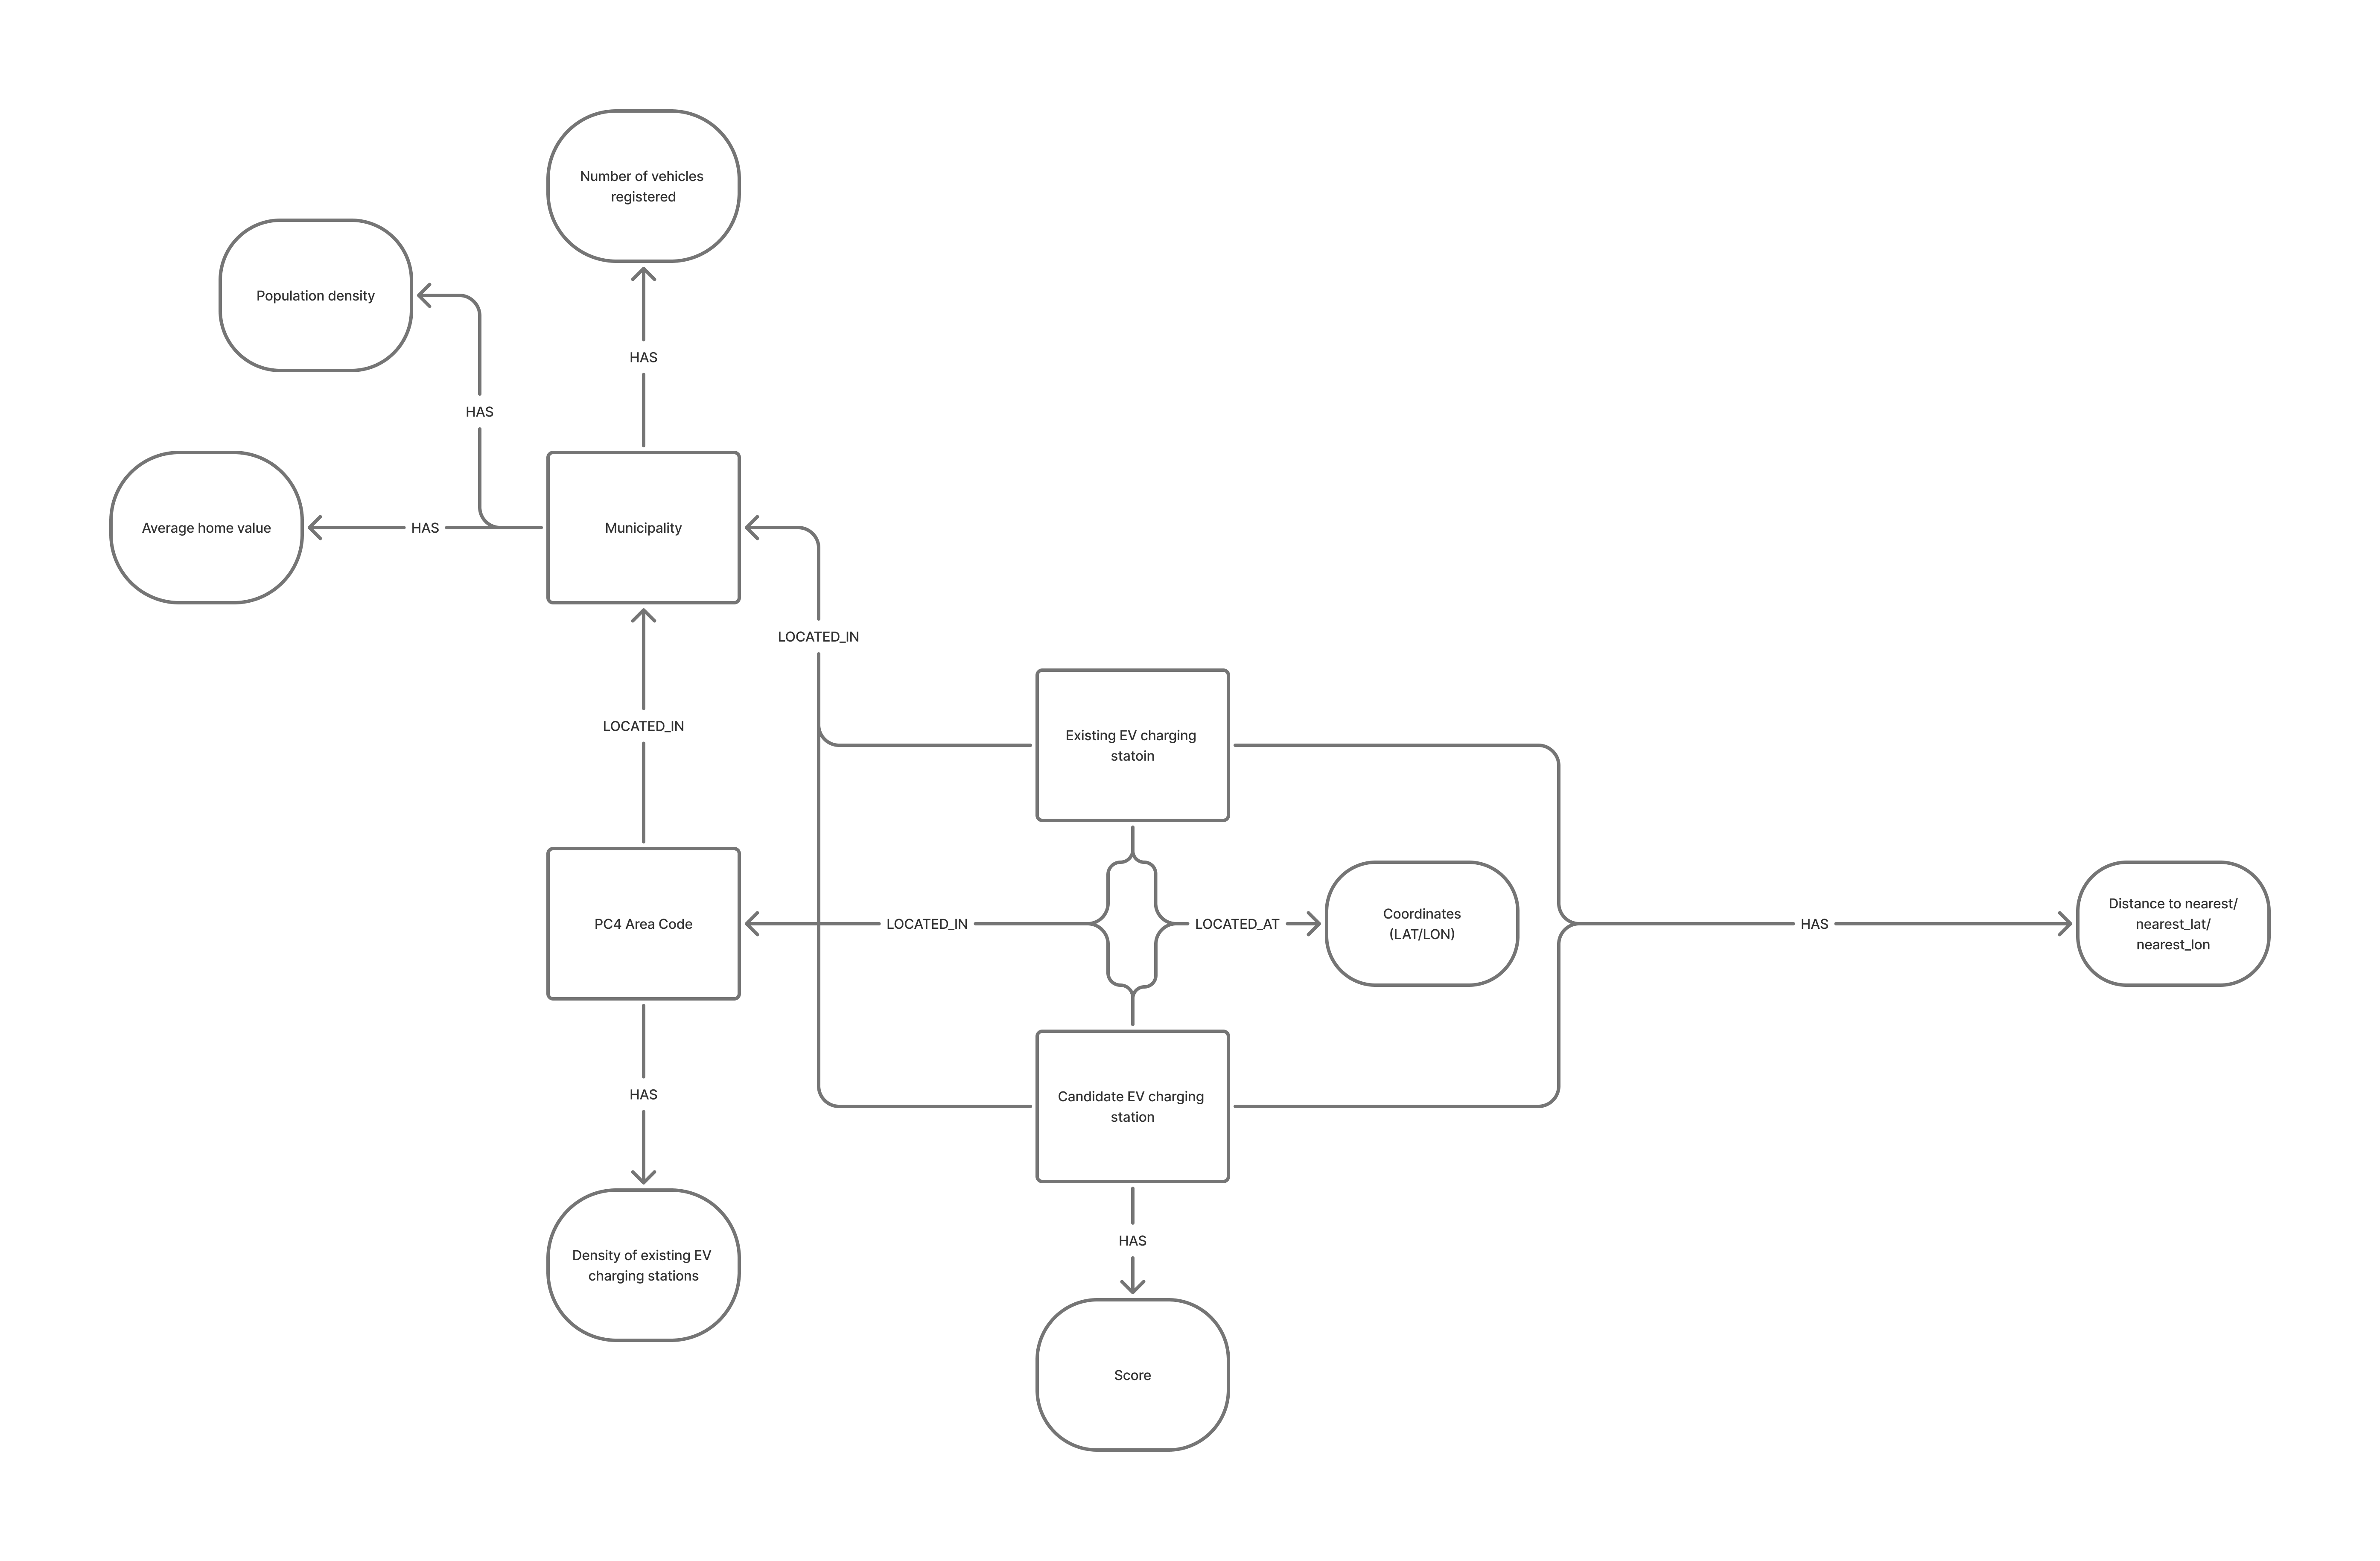
\includegraphics[width=\textwidth]{KnowledgeGraphGroup7.png}
	\caption{Structure of the knowledge graph, showing node types, key relationships, and important attributes used for scoring and querying.}
	\label{fig:graph_structure}
\end{figure}

\subsubsection{Illustrative Example}

Figure~\ref{fig:graph_excerpt_example} provides a concrete example from our knowledge graph to illustrate the structure and the relationships between nodes clearly. This excerpt highlights one existing EV charging station (\texttt{EXISTING1}), one candidate location (\texttt{CANDIDATE1}), their shared PC4 area (3273), and the associated municipality (Hoeksche Waard). Key properties such as population density, average home value, number of registered vehicles, charger density, proximity measures, and the candidate's computed suitability score are explicitly shown.

In this representation, entity nodes are depicted as rectangles, while rounded shapes denote property values.

\begin{figure}[htbp]
	\centering
	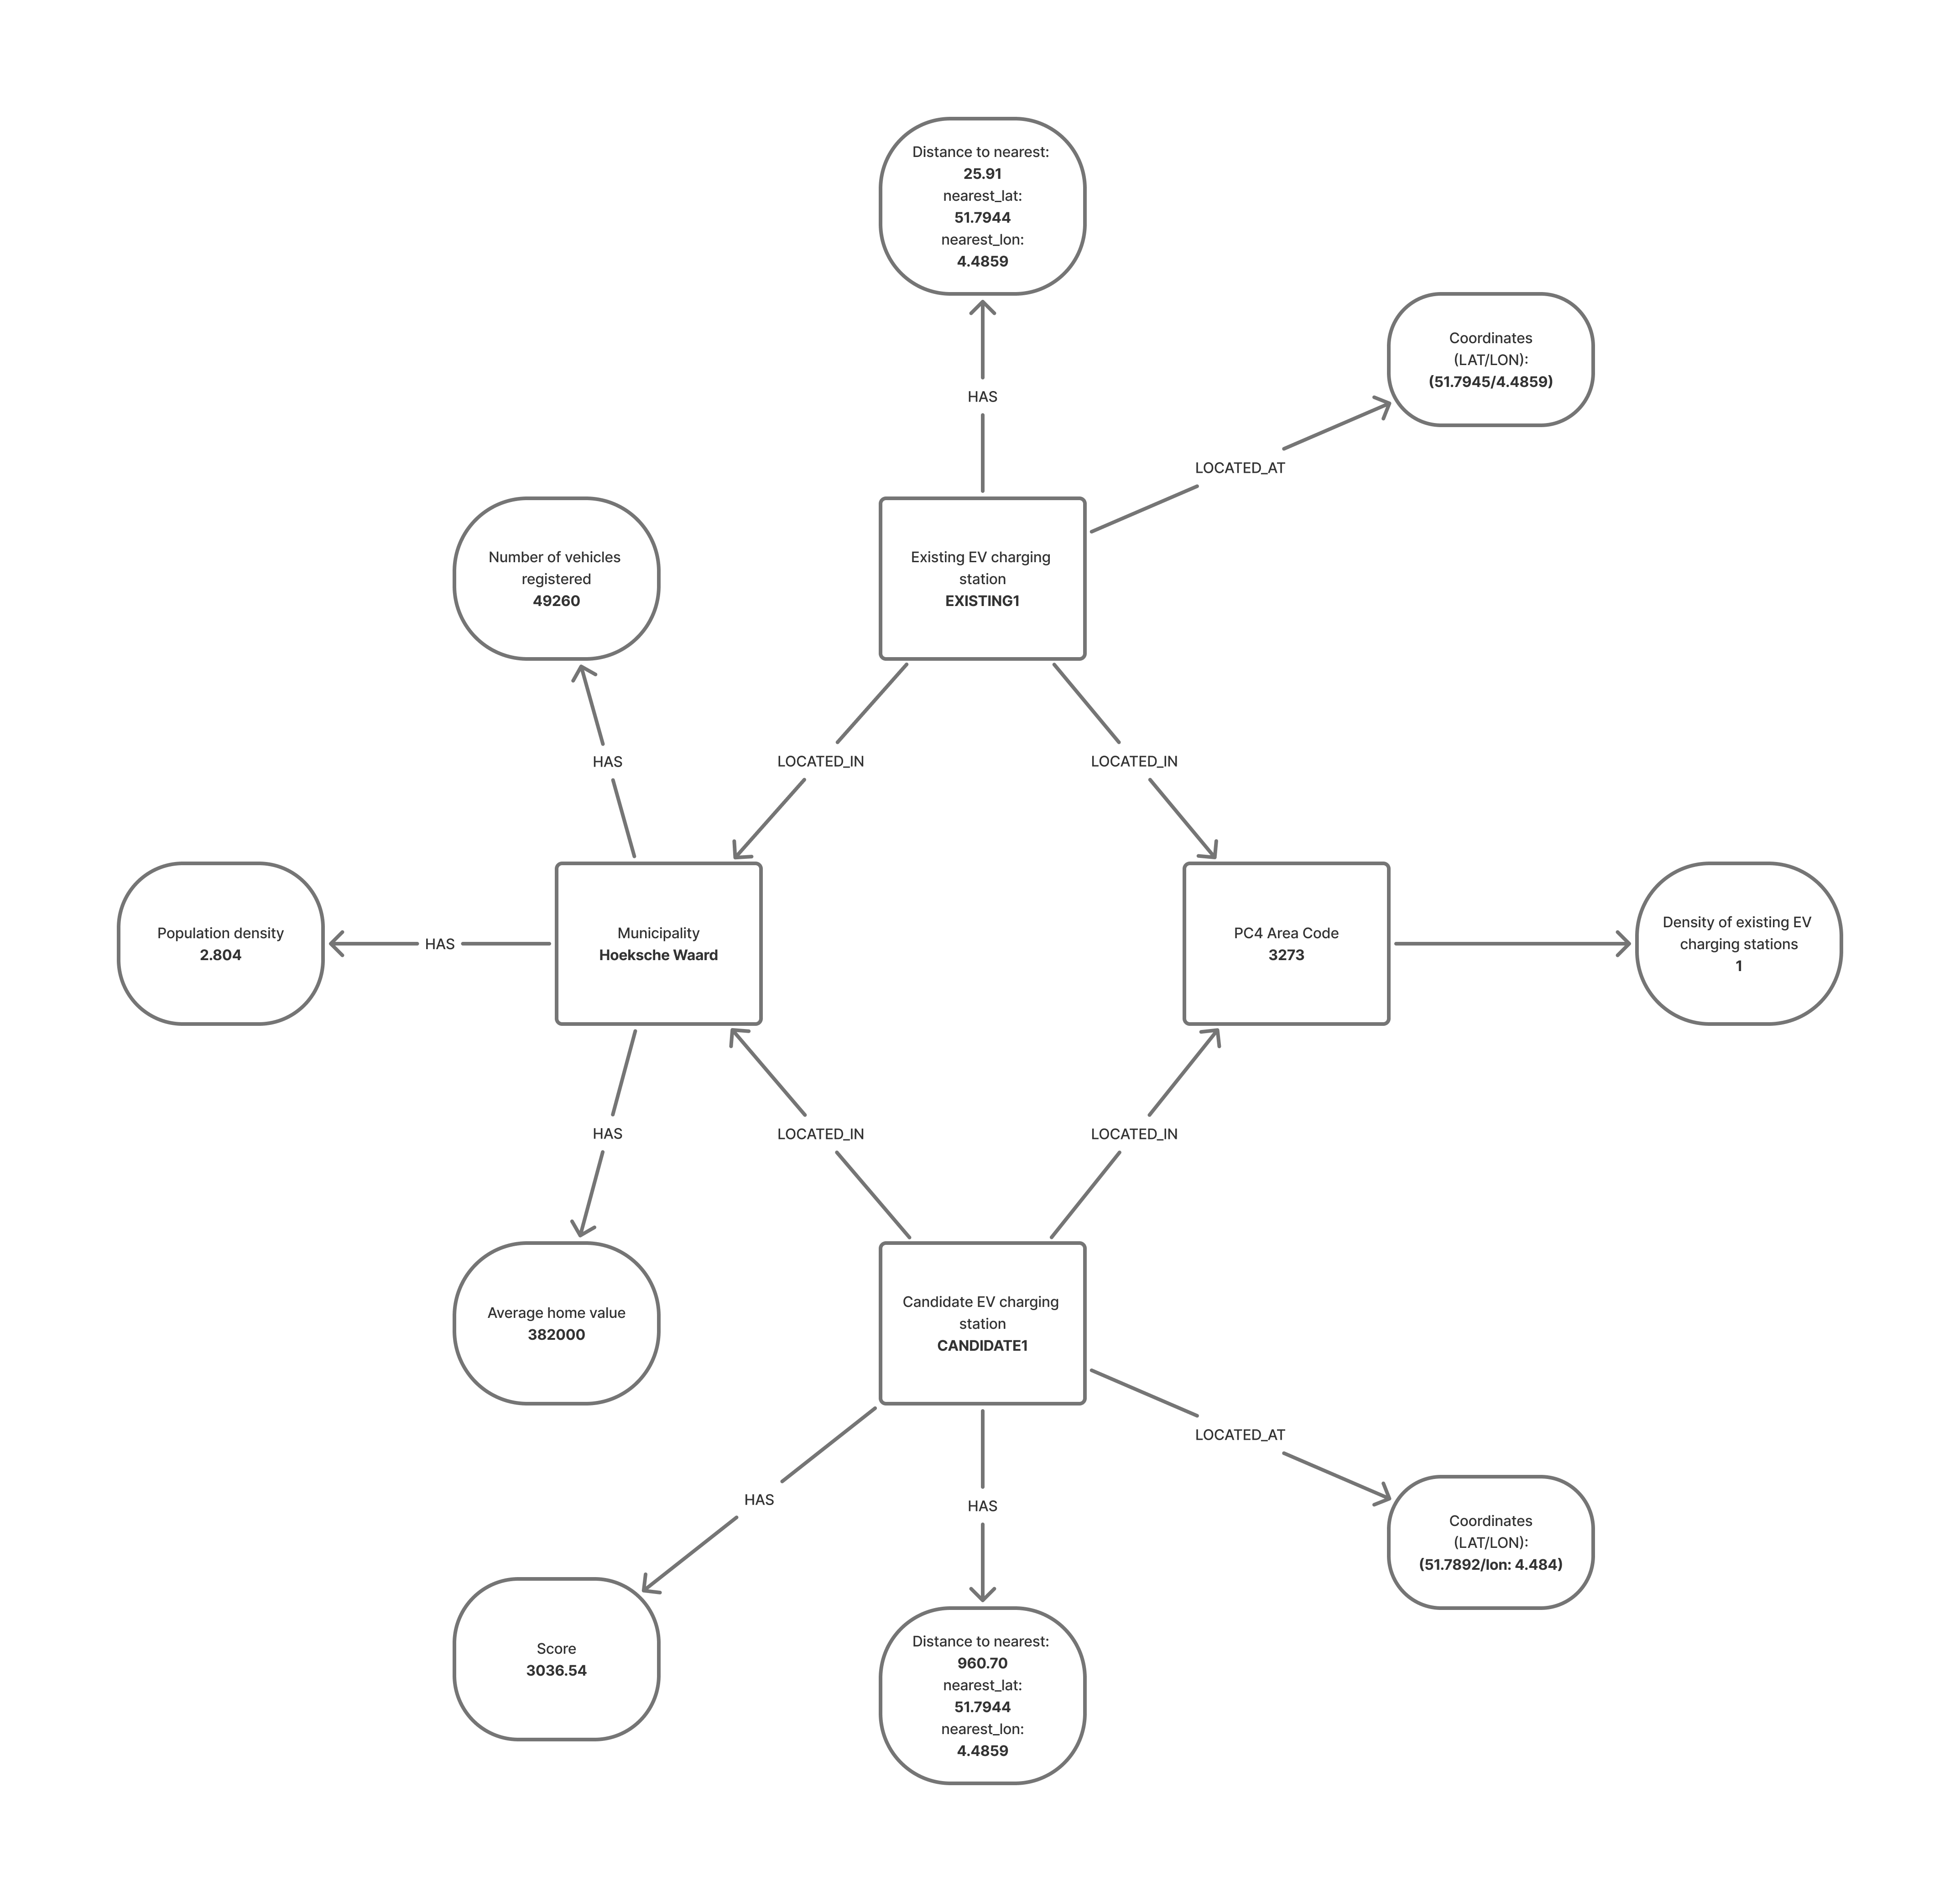
\includegraphics[width=\textwidth]{ExampleKnowledgeGraph.png}
	\caption{Illustrative subgraph excerpt showing relationships and key properties for a candidate EV charging location, an existing EV charging station, their common PC4 area, and associated municipality. Rounded nodes represent properties, rectangular nodes represent entities, and labeled arrows denote relationship types.}
	\label{fig:graph_excerpt_example}
\end{figure}

\subsection{Client-Oriented Queries and Scoring Logic}

The primary objective of the knowledge graph is to assist the client in identifying optimal locations for establishing new electric vehicle (EV) charging stations. To achieve this goal, queries were developed that leverage a domain-specific scoring mechanism. These queries are designed either to retrieve candidate locations based on precomputed scores or to facilitate the extraction of relevant data for external score computations.

\subsubsection{Overview of the Scoring Mechanism}

Each \texttt{CandidateLocation} within the knowledge graph is assigned a numerical score indicative of its suitability for hosting a new EV charging station. This score is computed externally, for instance, through a Jupyter notebook, and subsequently stored in the Neo4j database as a node property. The score is derived from a weighted combination of various factors related to both the candidate node itself and the associated administrative regions:

\begin{itemize}
	\item \textbf{Population Density} of the municipality
	\item \textbf{Average Home Value}, serving as a proxy indicator for income levels
	\item \textbf{Vehicle Ownership Rate}, defined as the number of vehicles per inhabitant
	\item \textbf{Existing Charger Density} within the relevant PC4 area
	\item \textbf{Distance to Nearest Charging Station}, with greater distances implying higher potential demand
\end{itemize}

The scoring formula is conceptually represented as follows:

\[
	\text{score} = w_1 \times \text{population\_density} + w_2 \times \text{home\_value} + w_3 \times \text{vehicles\_per\_capita}
	+ w_4 \times \frac{1}{\text{charger\_density}} + w_5 \times \text{distance\_to\_nearest}
\]

The weights ($w_1$ to $w_5$) were empirically determined to appropriately balance socio-economic and infrastructural considerations. For the standard scenario utilized in this analysis, the specific weights applied were:

\begin{verbatim}
closest_charging_location:       3
EV charger density (inverted):   5
Average home value:              0.5
Number of vehicles:              2
Population density:              1
\end{verbatim}

Upon computation, the scores were integrated into the knowledge graph by assigning them as properties to the respective \texttt{CandidateLocation} nodes.

\subsubsection{Querying Optimal Locations}

With the scores readily available in the graph, Cypher queries can efficiently retrieve the highest-ranking candidate locations within specific municipalities. For instance, to identify the top candidate locations within Rotterdam:

\begin{lstlisting}[style=cypherStyle,caption={Retrieve top 5 candidate locations in Rotterdam}label={lst:rotterdam_top5}]
MATCH (c:CandidateLocation)-[:LOCATED_IN]->(m:Municipality)
WHERE m.name = 'Rotterdam'
RETURN c.lat, c.lon, c.score
ORDER BY c.score DESC
LIMIT 5;
\end{lstlisting}

Clients may also apply filters based on charger density, population density, or proximity criteria. An example query demonstrating this capability is:

\begin{lstlisting}[style=cypherStyle,caption={Filtered query example}, label={lst:filtered_query}]
MATCH (c:CandidateLocation)-[:LOCATED_IN]->(p:PC4Area)-[:LOCATED_IN]->(m:Municipality)
WHERE p.density < 0.01 AND m.population_density > 1000
RETURN c.lat, c.lon, c.score
ORDER BY c.score DESC
LIMIT 5;
\end{lstlisting}

To retrieve the top 10 candidate locations across the entire dataset irrespective of administrative boundaries, the following query is recommended:

\begin{lstlisting}[style=cypherStyle,caption={Top 10 locations across the entire dataset}, label={lst:top10_global}]
MATCH (c:CandidateLocation)
RETURN c.lat, c.lon, c.score
ORDER BY c.score DESC
LIMIT 10;
\end{lstlisting}

\section{Other important aspects of the dataset and knowledge graph}

\question{\subsubsection*{Are there important aspects of the dataset/knowledge graph highlighted by the frameworks of Pushkarna et al.\ \cite{pushkarna} and Paullada et al.\ \cite{Paullada}, which are not covered in the sections above?  If so, note them here.}}

While earlier sections detail many critical aspects of our knowledge graph, applying the transparency frameworks proposed by Pushkarna et al.~\cite{pushkarna} and Paullada et al.~\cite{Paullada} provides additional insights for responsible data management and usage.

\textbf{1. Uncertainty and Known Unknowns (Pushkarna et al.~\cite{pushkarna})}
Our knowledge graph integrates data from official and crowd-sourced sources, such as OpenStreetMap and OpenChargeMap. Despite briefly acknowledging potential noise and duplication in charger location data, we have not explicitly documented uncertainties or potential inaccuracies. Pushkarna et al. argue that clearly articulating these uncertainties is essential for stakeholders to accurately assess risks and reliability. Future iterations could include explicit metadata annotations or confidence metrics, particularly for crowd-sourced contributions.

\textbf{2. Dataset Lifecycle and Updates (Pushkarna et al.~\cite{pushkarna})}
While mechanisms for updating our data sources, such as OpenStreetMap and OpenChargeMap, are described, our current documentation lacks details about versioning, archiving, and the traceability of historical data states. Pushkarna et al. emphasize the importance of lifecycle transparency, recommending clear documentation of dataset updates, version control practices, and records of changes to ensure longitudinal reproducibility and clarity for future decision-making processes.

\textbf{3. Motivation and Framing (Paullada et al.~\cite{Paullada})}
Paullada et al. highlight how dataset framing influences the problems addressed and solutions proposed. Our project explicitly frames the task around optimizing profitability for EV charger placement, inherently adopting an economic perspective. Alternative framings, such as prioritizing sustainability or equitable access, could shift the selection and weighting of factors within our model. Recognizing this inherent framing bias is important for stakeholders to critically evaluate the resulting recommendations.

\question{\subsubsection*{How are the visualisations created and how can they be used to asnwer the research question?}}

The visualisations are created in Python using Pydeck and Streamlit.

Each visualisation serves its own purpose and we have listed them as follows:
\begin{enumerate}
	\item Candidate Point Map: Displays the top n locations to build a new EV Charger in Zuid-Holland. Green represents a high score and Red represents a low score. Figure \ref{fig:point_map}
	\item Individual Candidate Map: For an individually chosen candidate location, displays all existing EV Chargers within a selectable number of kilometres of the candidate. Helps to visualise why a candidate may have a high or low score. Figure \ref{fig:point_map_ev_charger}
	\item PC4 Map: Interactive map to view the average score within each PC4 area. Helps to identify which PC4s in general have higher potential than others, allowing the client to focus their efforts. Figure \ref{fig:pc4}
	\item Table View: Helps the client to have a look at the raw data and view the individual statistics of each candidate. Figure \ref{fig:table_view}
\end{enumerate}

\begin{figure}[H]
	\centering
	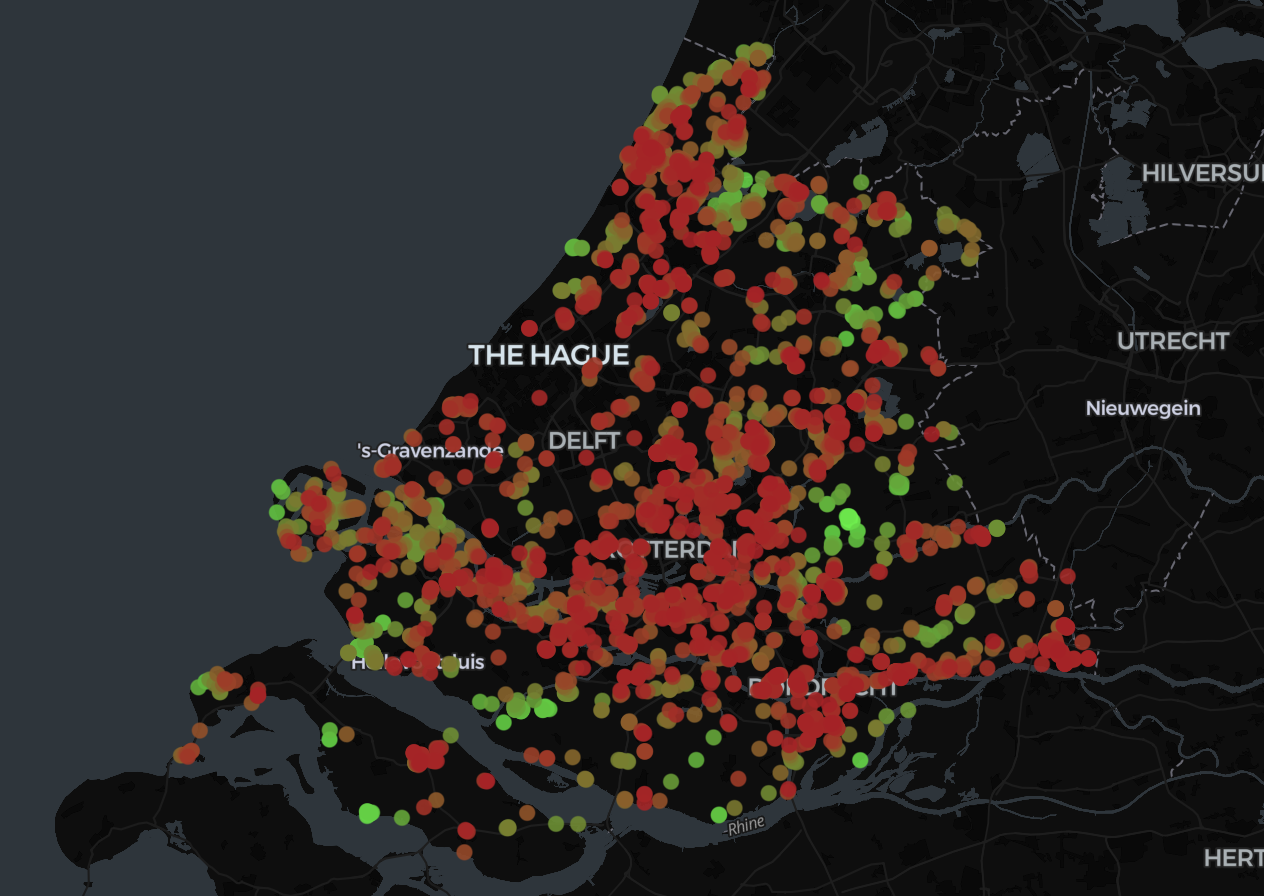
\includegraphics[width=0.75\linewidth]{point_map_view.png}
	\caption{Candidate Point Map}
	\label{fig:point_map}
\end{figure}

\begin{figure}[H]
	\centering
	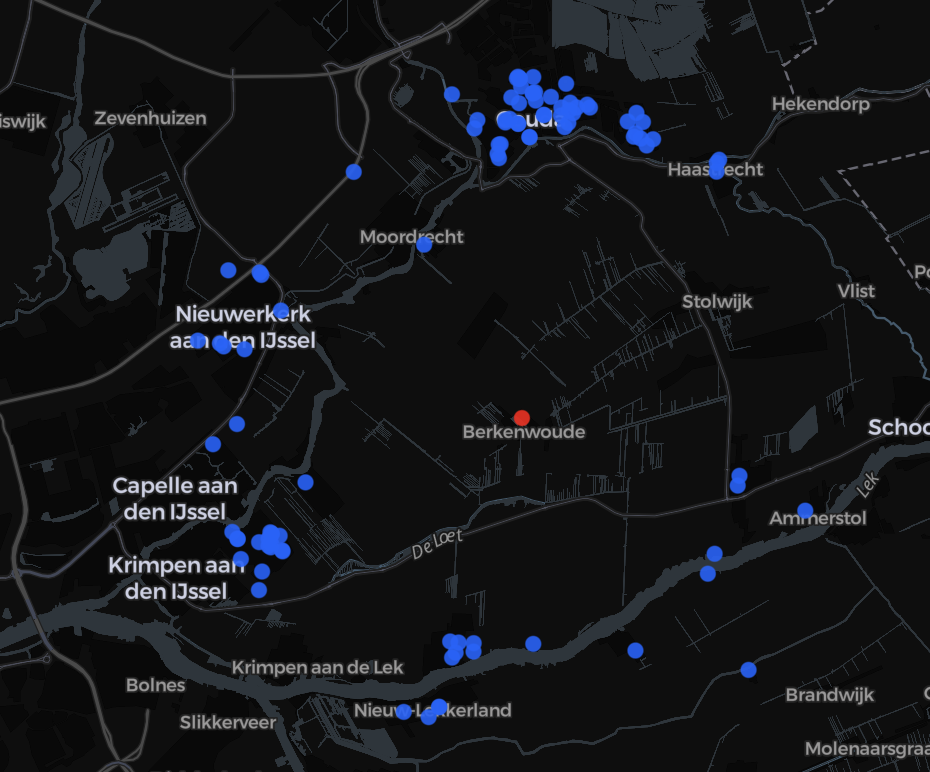
\includegraphics[width=0.75\linewidth]{point_map_view_ev_charger.png}
	\caption{Individual Candidate Map}
	\label{fig:point_map_ev_charger}
\end{figure}

\begin{figure}[H]
	\centering
	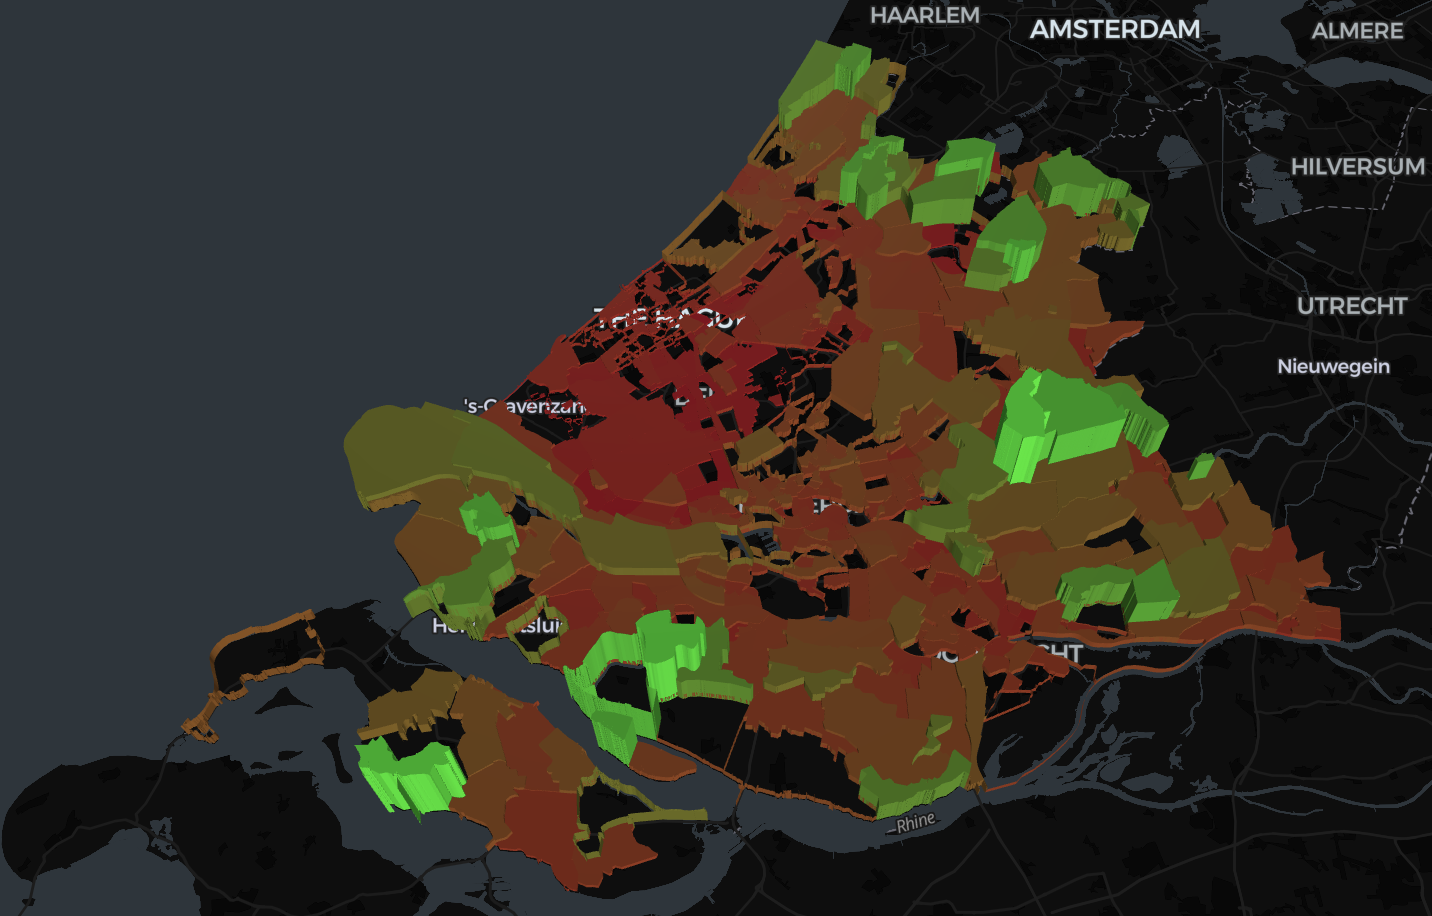
\includegraphics[width=0.75\linewidth]{pc4_map_view.png}
	\caption{PC4 Map}
	\label{fig:pc4}
\end{figure}

\begin{figure}[H]
	\centering
	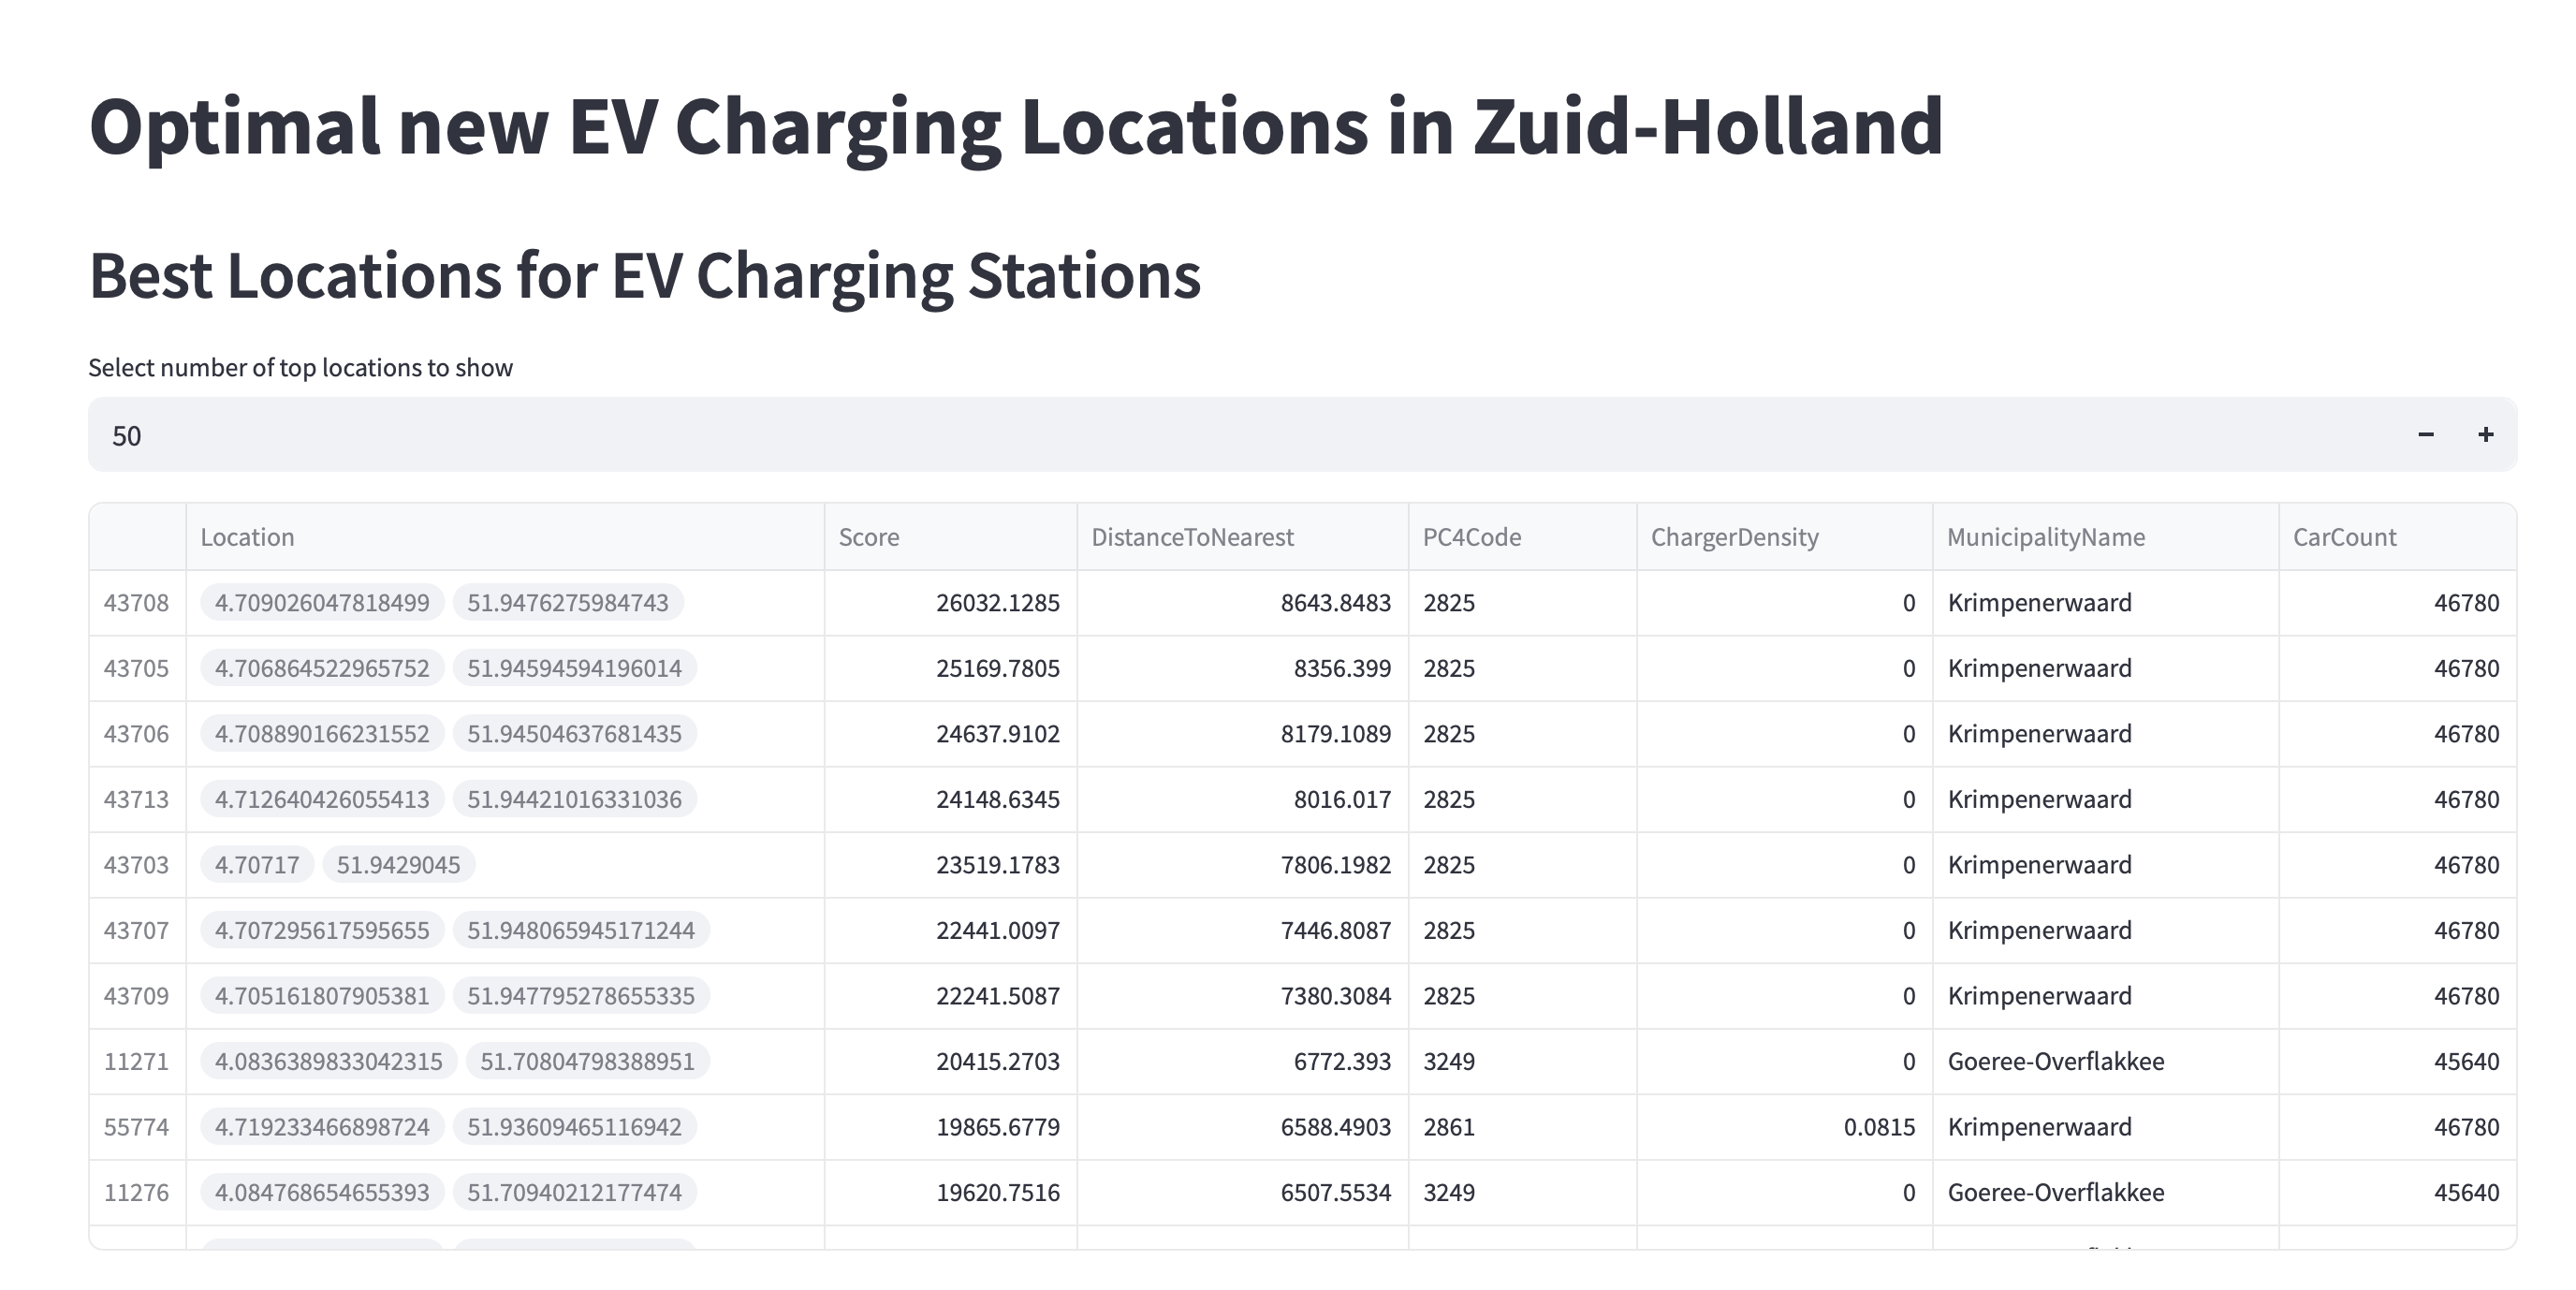
\includegraphics[width=0.75\linewidth]{table_view.png}
	\caption{Table View}
	\label{fig:table_view}
\end{figure}

\question{\subsubsection*{How will the knowledge graph be kept up to date?}}
Within the web ui, there is no way to indicate that a candidate has been turned into an EV Charger, or a new charger has been built. Therefore, the OSM and OCM APIs have to be called again. We have included a script in the Git repo with the steps for how to do it, but the relevant personnel have to be familiar with Python in order to do it.

\question{\subsubsection*{If the client wants to use different weights, how would those be applied?}}
Within the web ui, there is a page for rescoring, which can be accessed by the client to change the weights within the knowledge graph. This updates the score within the knowledge graph and thus all of our visualisations above.

\begin{figure}[H]
	\centering
	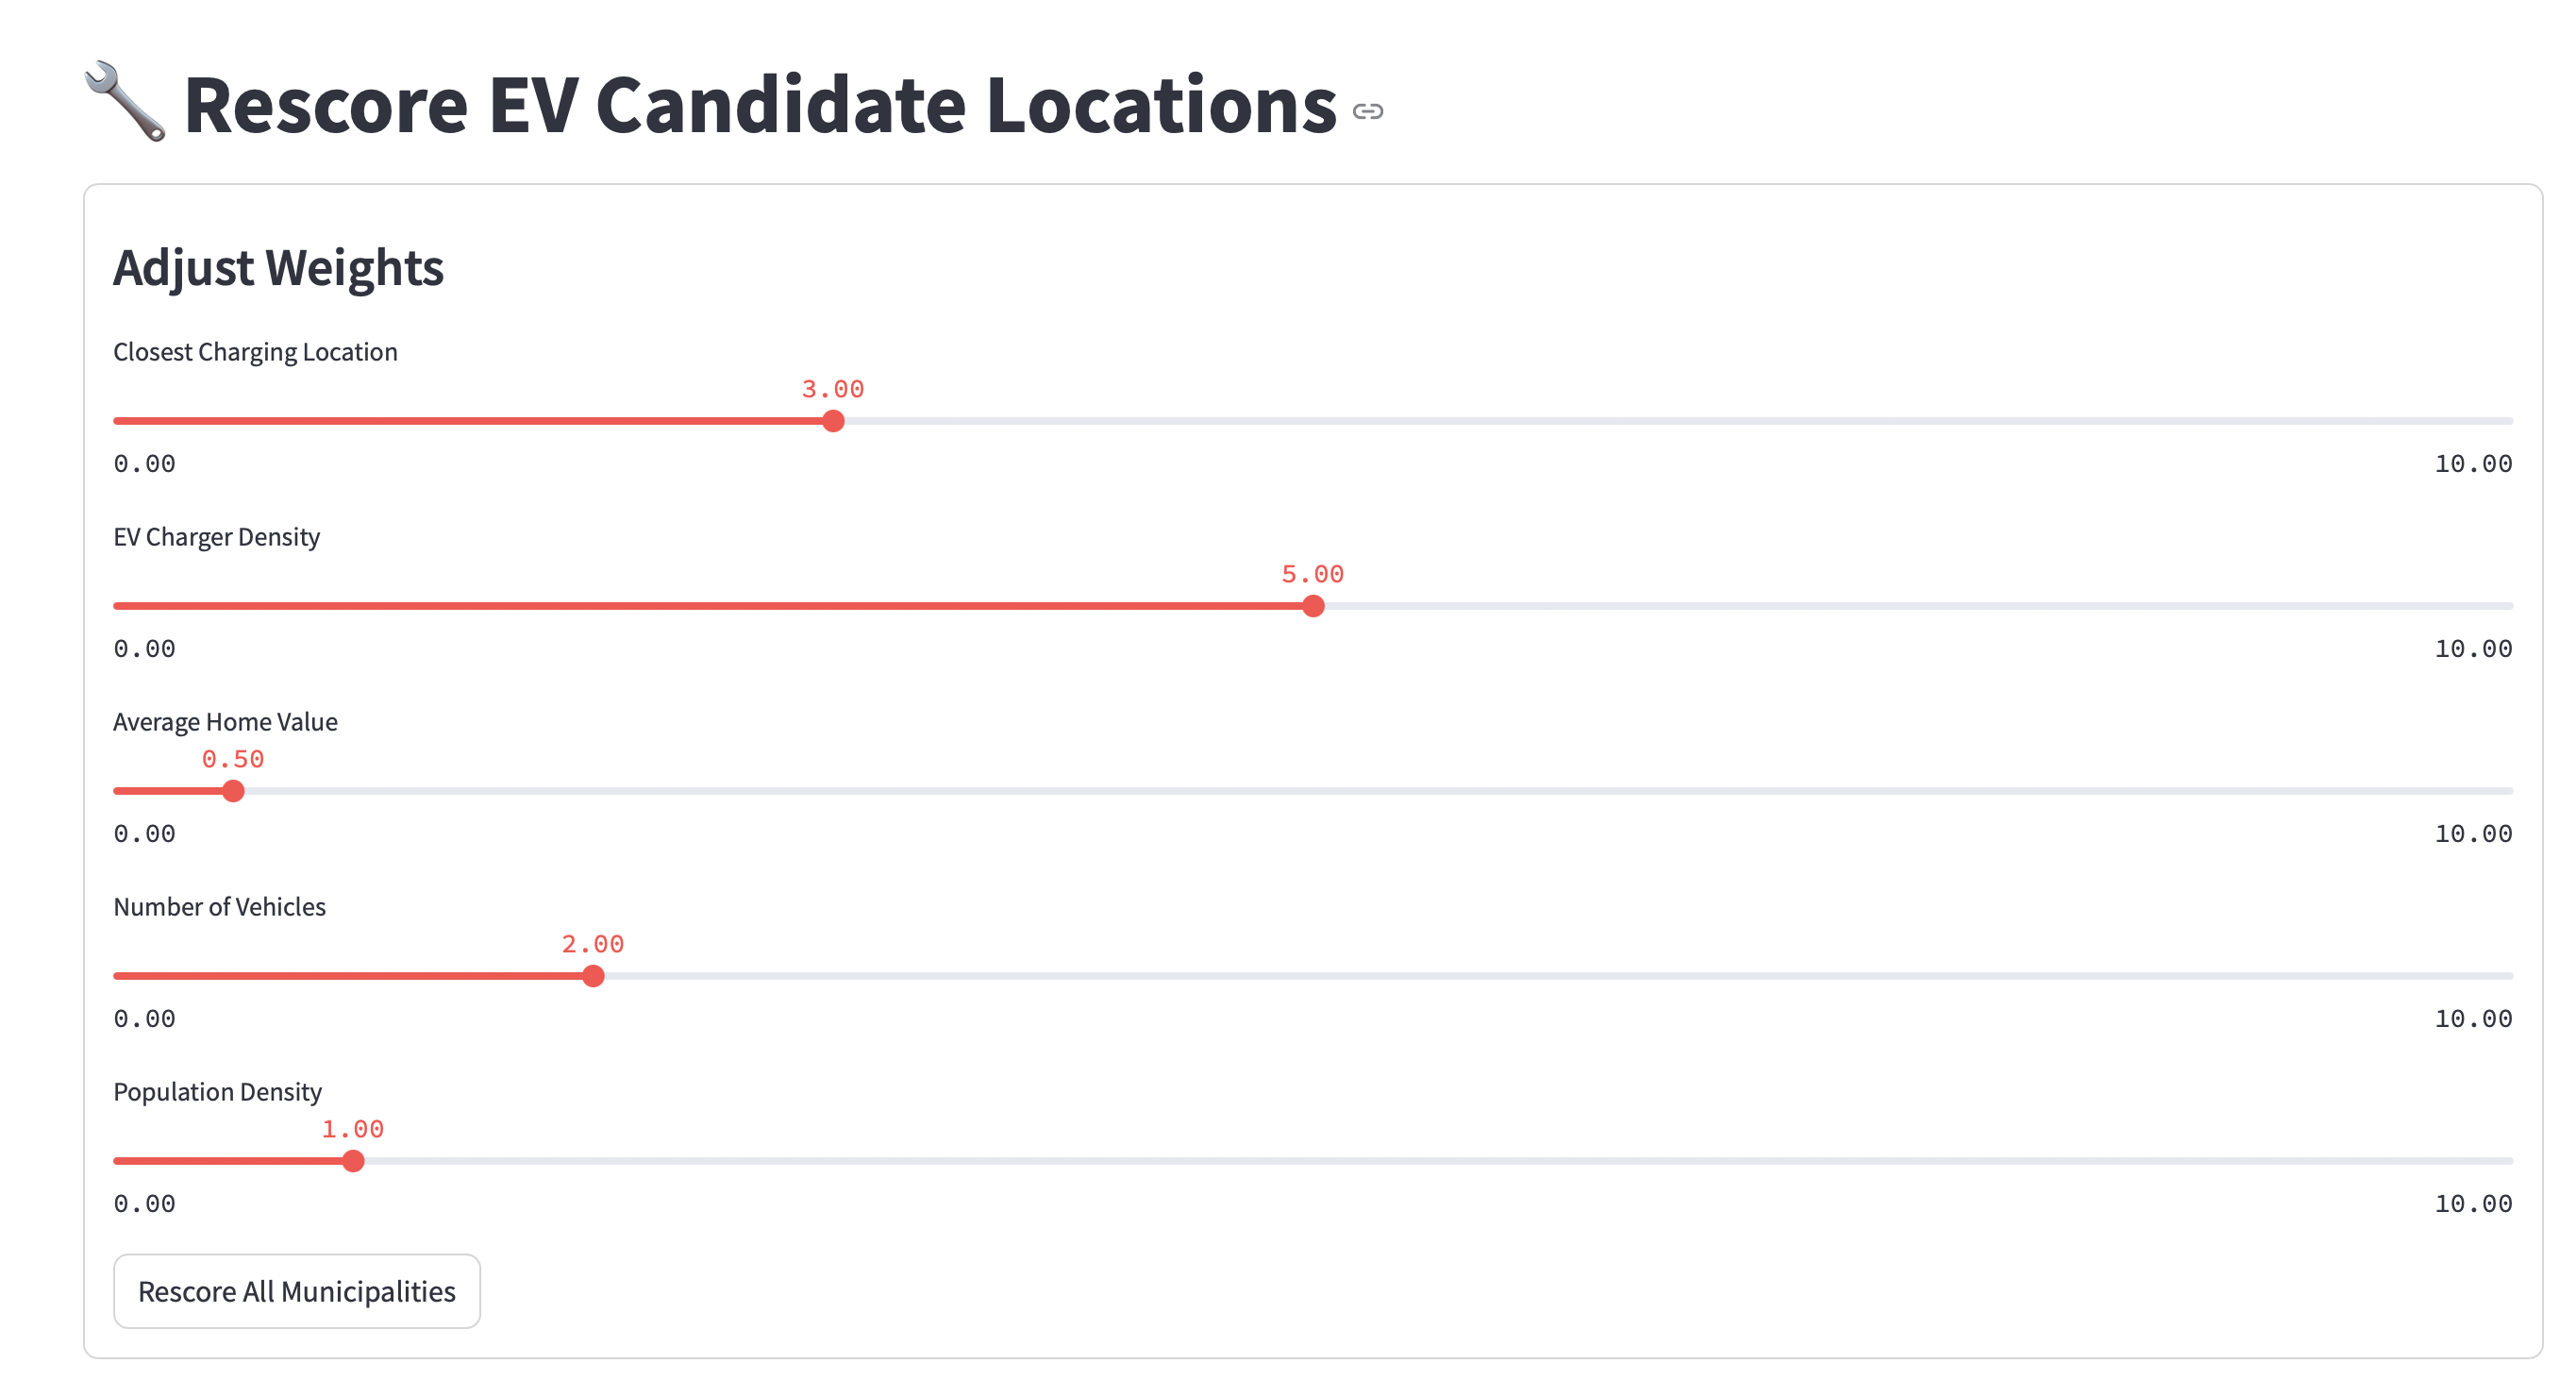
\includegraphics[width=0.75\linewidth]{rescore_view.png}
	\caption{Rescoring Page}
	\label{fig:rescore}
\end{figure}

\section*{Acknowledgment}

During the development of this project, various AI-based tools were employed in accordance with the AI policy:

\begin{itemize}
	\item \textbf{Text polishing}: The written content of this report was drafted by the authors. To enhance the readability, clarity, and quality of the language, we employed \textit{ChatGPT (OpenAI)} and \textit{DeepL Write} exclusively for the refinement of text that had previously been authored by us.

	\item \textbf{Code and project development}: We utilized AI-assisted development tools such as \textit{ChatGPT (OpenAI)}, \textit{GitHub Copilot}, \textit{CursorAI}, and \textit{Claude 4 Sonnet} to support code generation, debugging, and implementation. These tools were integrated into our workflow primarily for code suggestion and productivity enhancement.
\end{itemize}

All uses of AI have been limited to the above scope and are hereby fully disclosed in accordance with the course's AI usage policy.

\bibliographystyle{plain}
\bibliography{datasheet}

\appendix

\section{Client reflection on project outcomes}

As clients, we view the progress presented in this report to be adequate to answer our research question. The proposed solution can explicitly and directly answer the research question proposed. The key strengths are the integration of multiple datasets and the implementation of an actionable scoring mechanism. The integration of multiple datasets across the geospatial domain through mappings and data exchange makes the tool useful for our proposed area, while also being extensible towards larger regions when necessary. Furthermore, by providing a single weighted scoring system, we can gain a clear ranking based on a list of candidate locations and fine-tune the weights based on our own needs/priorities. The factors included in the score, such as existing charger density, average home value, and vehicle density, are some of the most relevant indicators to our business’s success and serve as a good baseline model.

The listed limitations are well-elaborated and already include some proposals for future work on the tool; it is easy for us, as stakeholders, to assess the project's risks and reliability accurately. By proposing future improvements, the project establishes a clear roadmap for enhancing its transparency and long-term viability.

In conclusion, your team has delivered a valuable analysis. The knowledge graph serves as a good working foundation for our data-driven expansion strategy. We thank you for your thoroughness, technical proficiency, clear communication, and alignment with our business objectives.

\section{Data Exchange Code} \label{appenxdix:data_exchange}
\begin{lstlisting}[style=pythonStyle,caption={Code for data exchange between OSM and OCM}, label={lst:data_exchange}]
import geopandas as gpd
import pandas as pd
from shapely.ops import nearest_points
from shapely.geometry import Point
from pyproj import CRS, Transformer

# Read data from pre-prepared files of OSM and OCM data
osm_charging_points = gpd.read_file('data/osm-charging_points-zuid-holland.geojson')
osm_charging_points = osm_charging_points.to_crs("EPSG:4326")
ocm_charging_points = gpd.read_file('data/ocm-charging-points-zuid-holland.json')
ocm_charging_points = ocm_charging_points.to_crs("EPSG:4326")

# combine the two datasets
combined_charging_points = pd.concat([osm_charging_points, ocm_charging_points], ignore_index=True)
combined_charging_points = combined_charging_points.drop_duplicates(subset=['lat', 'lon'])


# find the distance between each pair of points in the combined dataset
def generate_closest_points(points_gdf):
    # Convert the GeoDataFrame to a list of points in EPSG:3857
    transformer = Transformer.from_crs(CRS("EPSG:4326"), CRS("EPSG:3857"))
    result_gdf = points_gdf
    def find_nearest_charging_point(point, points_gdf):
        # excluide the point itself from the search
        points_gdf = points_gdf[points_gdf.geometry != point]
        nearest_geom = nearest_points(point, points_gdf.unary_union)[1]
        distance = Point(transformer.transform(point.x, point.y)).distance(Point(transformer.transform(nearest_geom.x, nearest_geom.y)))
        return nearest_geom.x, nearest_geom.y, distance
    result_gdf['nearest_lon'], result_gdf['nearest_lat'], result_gdf["distance_to_nearest"] = zip(*points_gdf.geometry.apply(lambda x: find_nearest_charging_point(x, points_gdf)))
    return result_gdf

# Return updated geopandas DataFrame
combined_charging_points = generate_closest_points(combined_charging_points)

# how many point within 2m of each other?
close_points = combined_charging_points[combined_charging_points['distance_to_nearest'] < 2]
print(f'Number of charging points within 2m of each other: {len(close_points)}')

# for each point whose nearest point is within 2m, remove that point, but do not remove the original point
removed_points = gpd.GeoDataFrame(columns=combined_charging_points.columns)
print(removed_points)
for point in close_points.iterrows():
    point = point[1]
    # if nearest_lon and nearest_lat are in the removed_points, skip this point since it has already been removed
    removed_points_check = removed_points[(removed_points['nearest_lon'] == point['lon']) &
                                         (removed_points['nearest_lat'] == point['lat'])]
    if not removed_points_check.empty:
        print(f'Skipping point {point["pc4_code"]} at ({point["lat"]}, {point["lon"]}) since it is already removed.')
        continue
    # otherwise, remove this point
    removed_points = pd.concat([removed_points, gpd.GeoDataFrame({'pc4_code': [point['pc4_code']], 'lat': [point['lat']], 'lon': [point['lon']], 'nearest_lon': [point['nearest_lon']], 'nearest_lat': [point['nearest_lat']], 'distance_to_nearest': [point['distance_to_nearest']], 'geometry': [Point(point['lon'], point['lat'])]})], ignore_index=True) 

# remove the points from the combined dataset
combined_charging_points = combined_charging_points[~combined_charging_points.geometry.isin(removed_points.geometry)]
print(f'Number of charging points after removing close points: {len(combined_charging_points)}')

# recalculate the nearest points
combined_charging_points = generate_closest_points(combined_charging_points)

# Verify that there are no other points within 2m
close_points = combined_charging_points[combined_charging_points['distance_to_nearest'] < 2]
print(f'Number of charging points within 2m of each other: {len(close_points)}')

# save the combined charging points to a file for uploading to neo4j in a seperate script
combined_charging_points.to_file('./data/combined-charging-points-zuid-holland.geojson', driver='GeoJSON')

\end{lstlisting}
\end{document}
